\documentclass{assignment}
\usepackage[pdftex]{graphicx} 
\usepackage{xcolor}
\definecolor{LightGray}{gray}{0.95}
%\usepackage{fancyvrb, minted} 
\usepackage[a4paper, margin = 2.5cm]{geometry} 
\usepackage[T1]{fontenc} 
% set figure path 
\graphicspath{figures}

\usepackage{amsmath, amsfonts, amssymb} 
\usepackage{hyperref, url}  
\usepackage{fancyhdr}
\usepackage{setspace}
\onehalfspacing

\usepackage{float}
\usepackage{subcaption}
\usepackage{listingsutf8}

\usepackage{xcolor}

\definecolor{codegreen}{rgb}{0,0.6,0}
\definecolor{codegray}{rgb}{0.5,0.5,0.5}
\definecolor{codepurple}{rgb}{0.58,0,0.82}
\definecolor{backcolour}{rgb}{0.95,0.95,0.92}

\lstdefinestyle{mystyle}{
    backgroundcolor=\color{backcolour},   
    commentstyle=\color{codegreen},
    keywordstyle=\color{magenta},
    numberstyle=\tiny\color{codegray},
    stringstyle=\color{codepurple},
    basicstyle=\ttfamily\footnotesize,
    breakatwhitespace=false,         
    breaklines=true,                 
    captionpos=b,                    
    keepspaces=true,                 
    numbers=left,                    
    numbersep=5pt,                  
    showspaces=false,                
    showstringspaces=false,
    showtabs=false,                  
    tabsize=2
}

\lstset{style=mystyle}

\student{Ahmet Akman 2442366}                             
\semester{Spring 2024}                            
\date{\today}                                   

\courselabel{EE449}          
\exercisesheet{Homework 3}{Report}  

\school{Middle East Technical University}        
\university{Electrical and Electronics Engineering}        

%%%%%%%%%%%%%%%%%%%%%%%%%%%%%%%%%%%%%%%%%%-DOCUMENT-%%%%%%%%%%%%%%%%%%%%%%%%%%%%%%%%%%%%%%%%%%%%

\begin{document}
\section{Questions}
\subsection{Agent: }
\subsection{Environment: }
\subsection{Reward: }
\subsection{Policy: }
\subsection{Exploration: }
\subsection{Exploitation: }


\section{Experimental Work}
\subsection{Temporal Difference Learning Default Parameters}

\subsection{Q-Learning Default Parameters}

\begin{figure}[H]
    \begin{subfigure}{0.3\textwidth}
        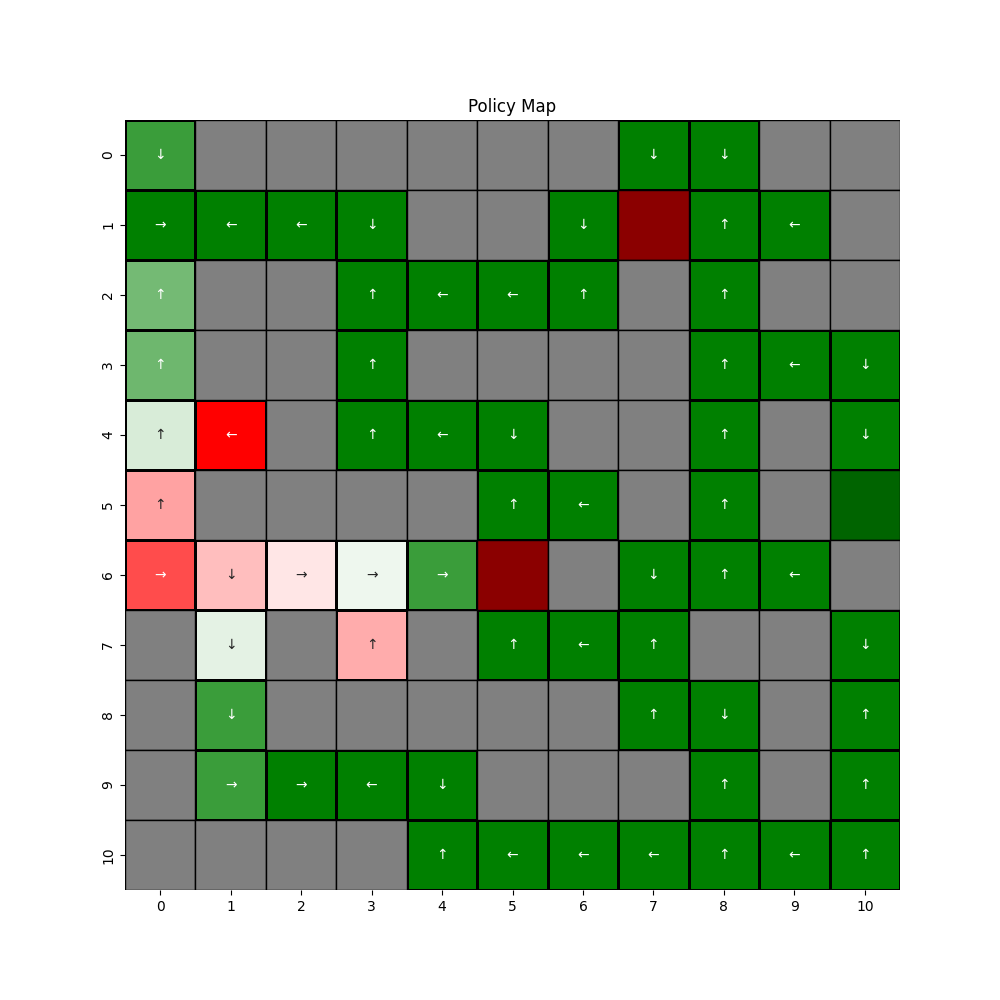
\includegraphics[width=\textwidth]{figures/policy_q/default/policy_alpha_0.1_gamma_0.95_epsilon_0.2_iteration_1.png}
    \caption{Episode 1.}
    \end{subfigure}\hfill
    \begin{subfigure}{0.3\textwidth}
        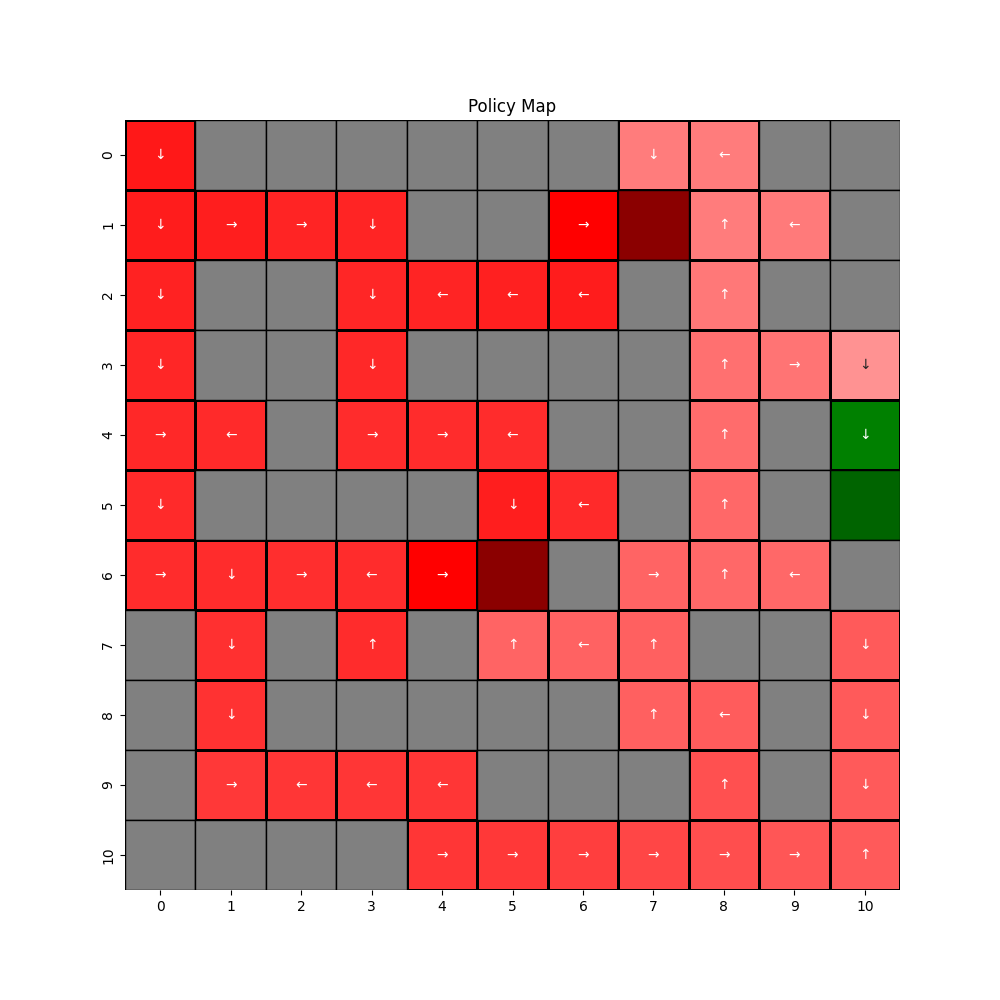
\includegraphics[width=\textwidth]{figures/policy_q/default/policy_alpha_0.1_gamma_0.95_epsilon_0.2_iteration_50.png}
    \caption{Episode 50}
    \end{subfigure}\hfill
    \begin{subfigure}{0.3\textwidth}
        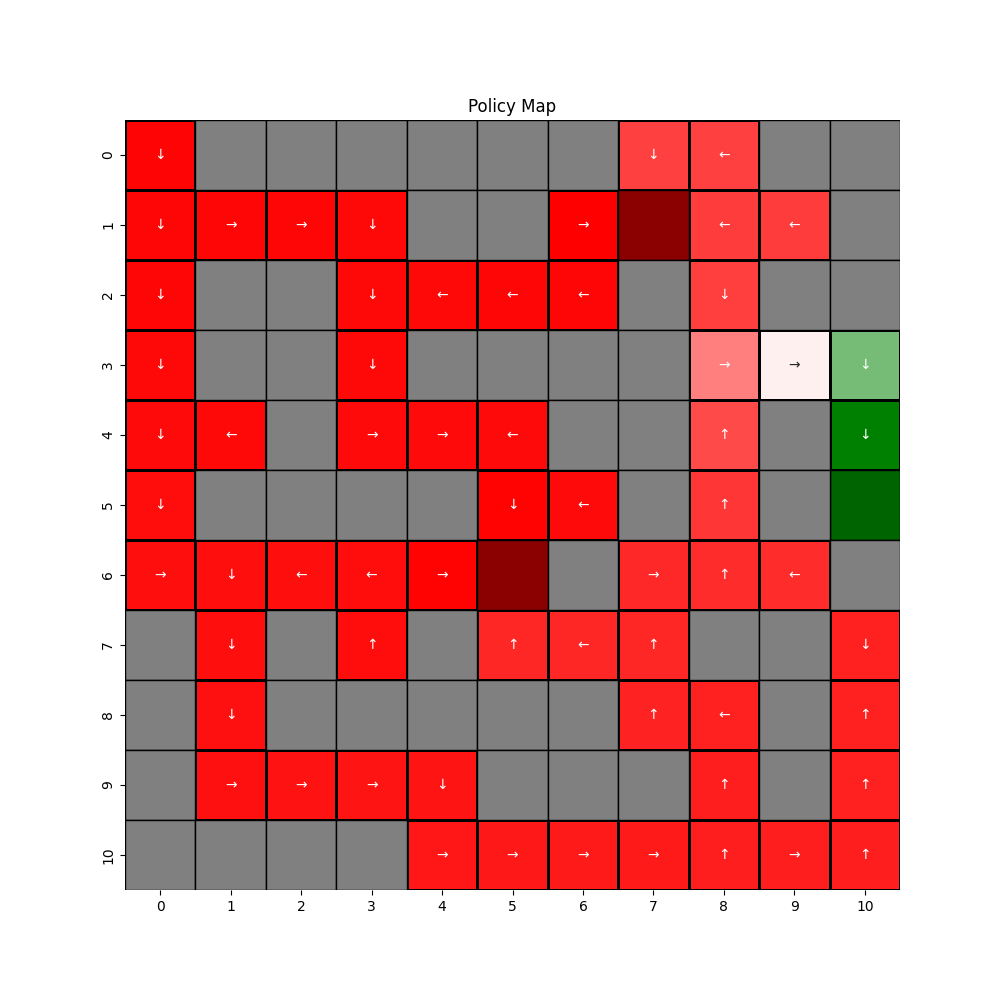
\includegraphics[width=\textwidth]{figures/policy_q/default/policy_alpha_0.1_gamma_0.95_epsilon_0.2_iteration_100.png}
    \caption{Episode 100}
    \end{subfigure}
    \begin{subfigure}{0.3\textwidth}
        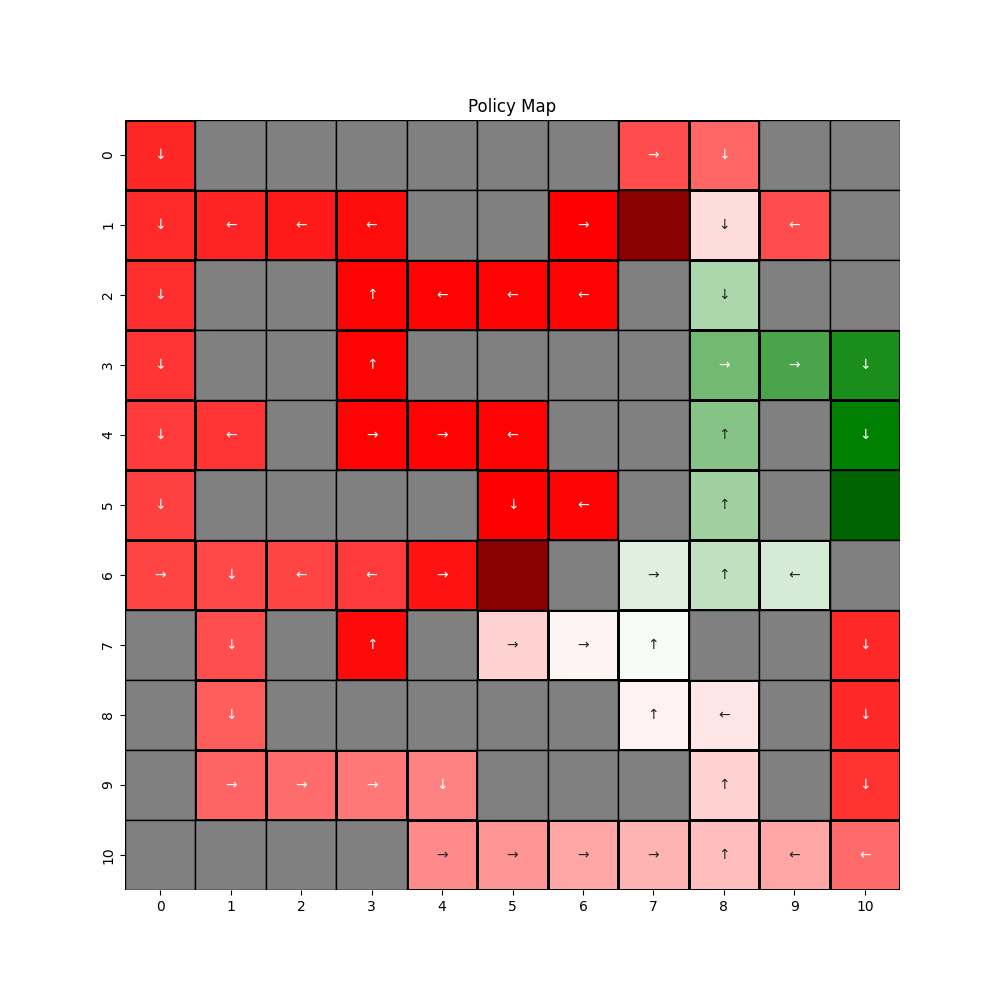
\includegraphics[width=\textwidth]{figures/policy_q/default/policy_alpha_0.1_gamma_0.95_epsilon_0.2_iteration_1000.png}
    \caption{Episode 1000.}
    \end{subfigure}\hfill
    \begin{subfigure}{0.3\textwidth}
        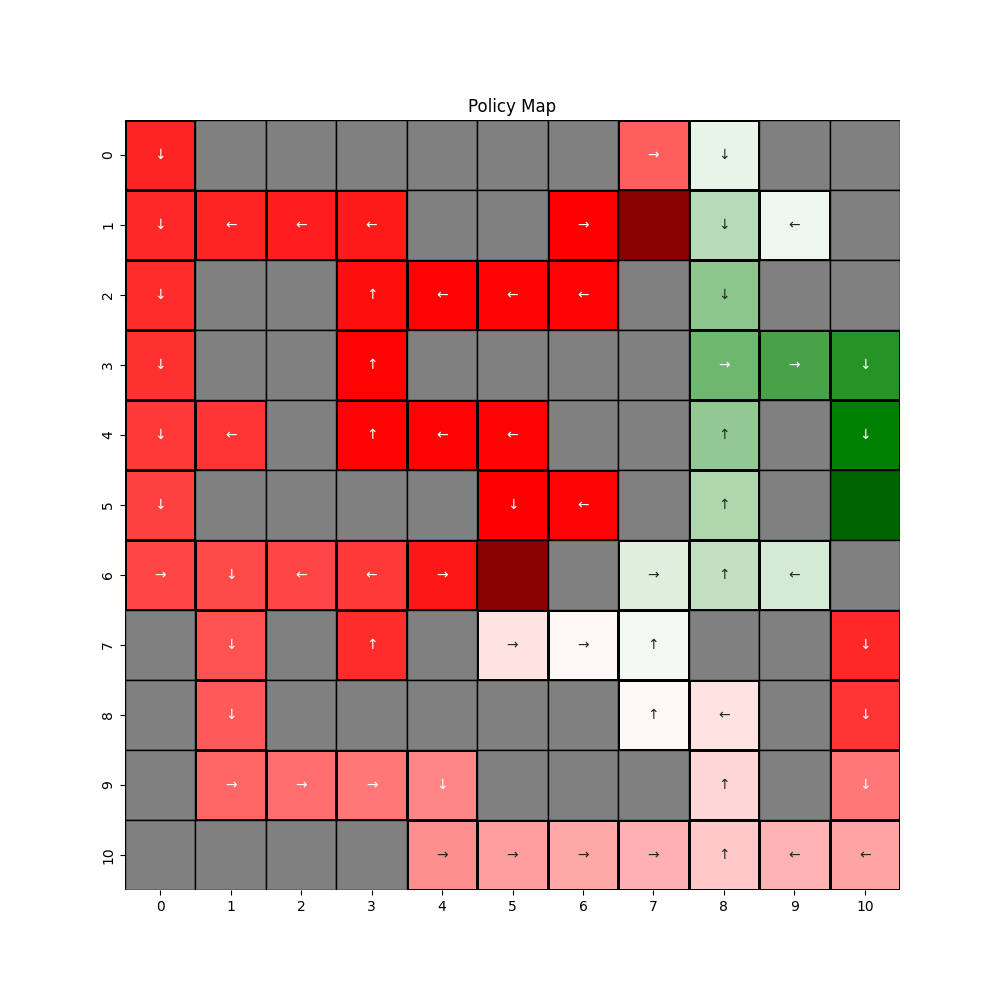
\includegraphics[width=\textwidth]{figures/policy_q/default/policy_alpha_0.1_gamma_0.95_epsilon_0.2_iteration_5000.png}
    \caption{Episode 5000}
    \end{subfigure}\hfill
    \begin{subfigure}{0.3\textwidth}
        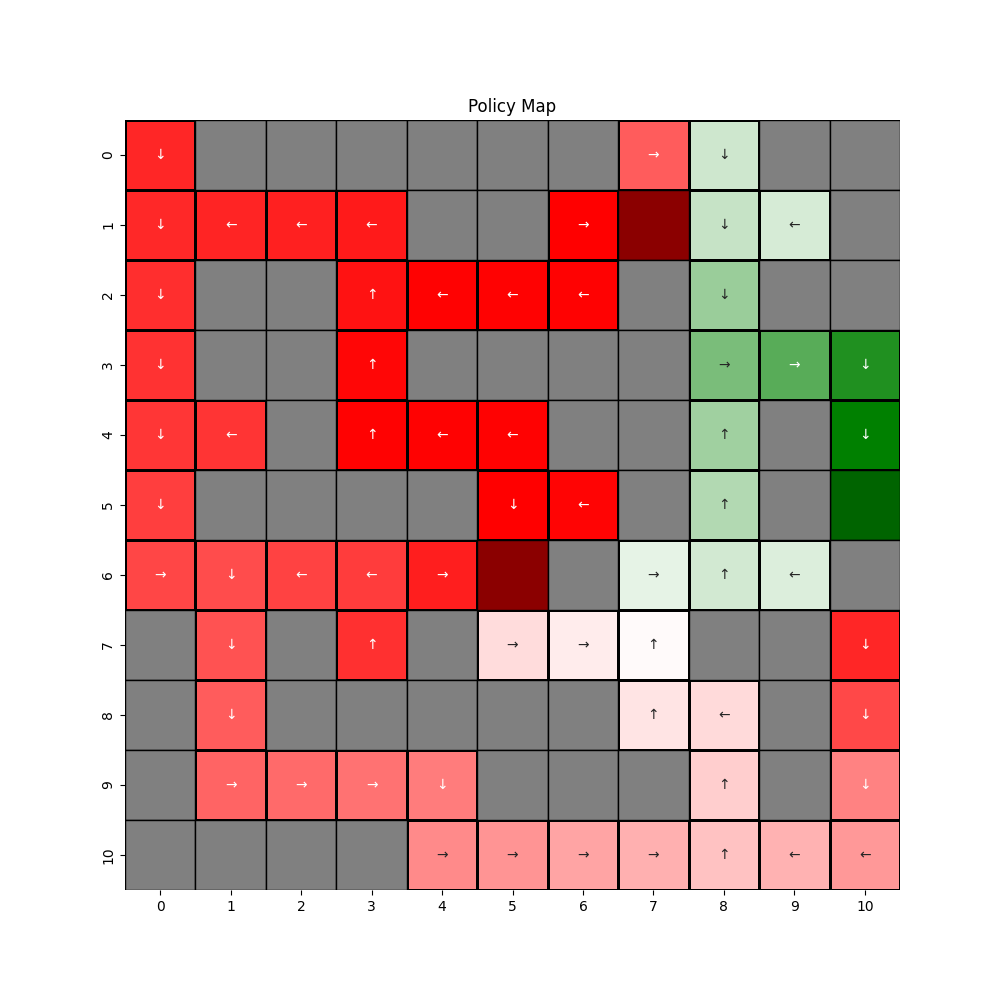
\includegraphics[width=\textwidth]{figures/policy_q/default/policy_alpha_0.1_gamma_0.95_epsilon_0.2_iteration_10000.png}
    \caption{Episode 10000}
    \end{subfigure}
    \caption{Evolution of policy maps throughout episodes.}
    \label{fig:default_q_learning_policy}
\end{figure}




\begin{figure}[H]
    \begin{subfigure}{0.3\textwidth}
        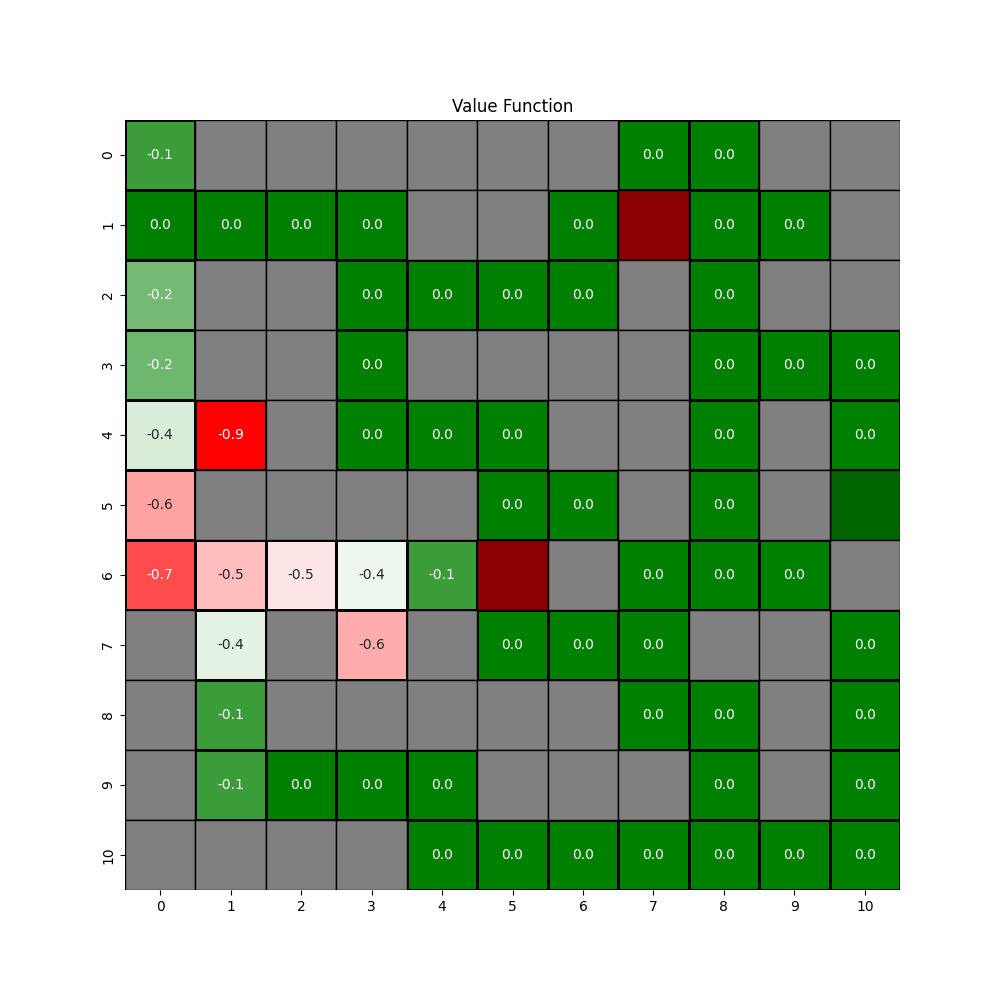
\includegraphics[width=\textwidth]{figures/value_q/default/value_function_alpha_0.1_gamma_0.95_epsilon_0.2_iteration_1.png}
    \caption{Episode 1.}
    \end{subfigure}\hfill
    \begin{subfigure}{0.3\textwidth}
        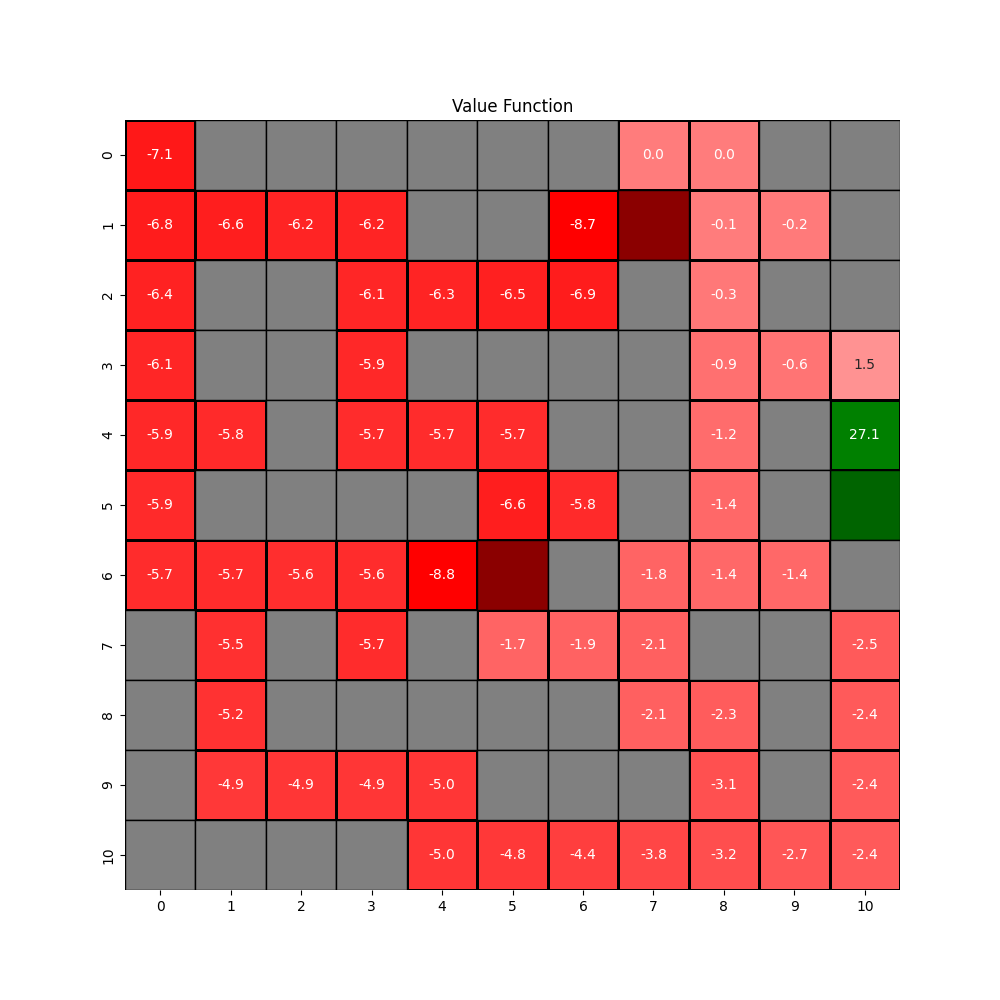
\includegraphics[width=\textwidth]{figures/value_q/default/value_function_alpha_0.1_gamma_0.95_epsilon_0.2_iteration_50.png}
    \caption{Episode 50}
    \end{subfigure}\hfill
    \begin{subfigure}{0.3\textwidth}
        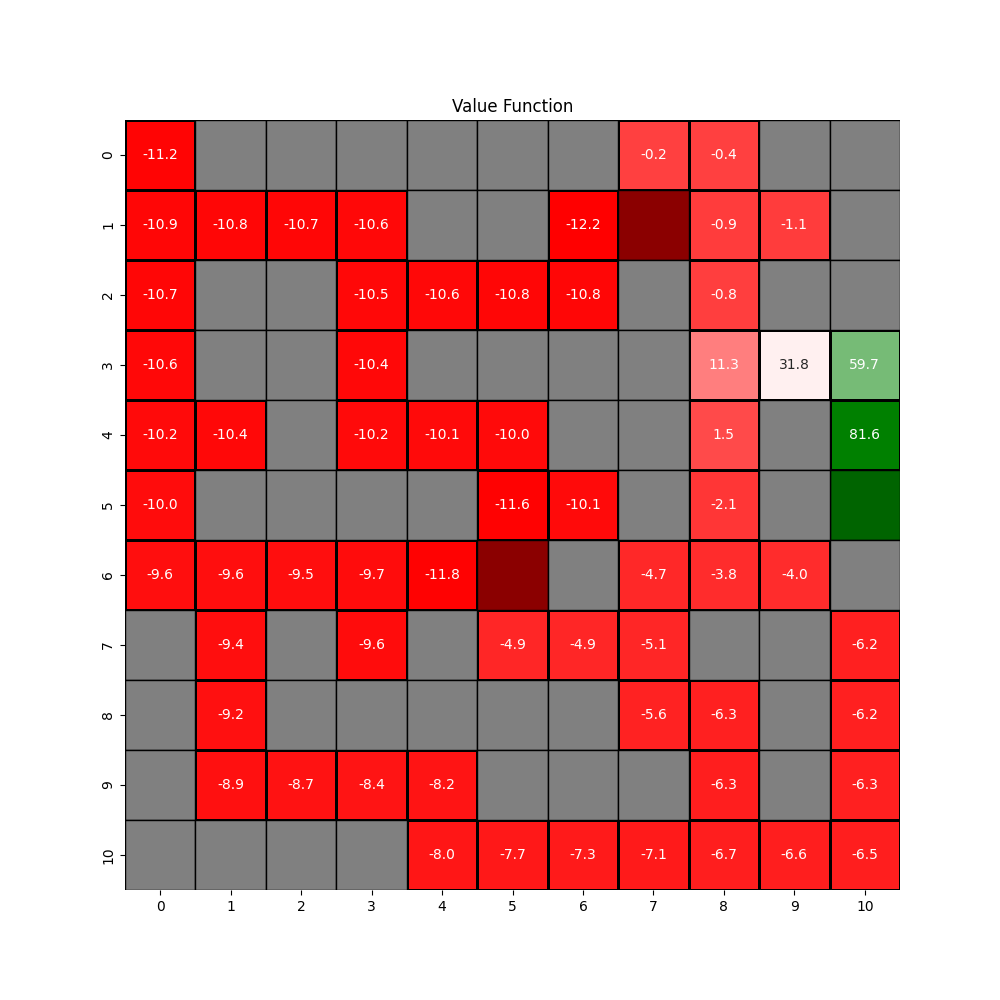
\includegraphics[width=\textwidth]{figures/value_q/default/value_function_alpha_0.1_gamma_0.95_epsilon_0.2_iteration_100.png}
    \caption{Episode 100}
    \end{subfigure}
    \begin{subfigure}{0.3\textwidth}
        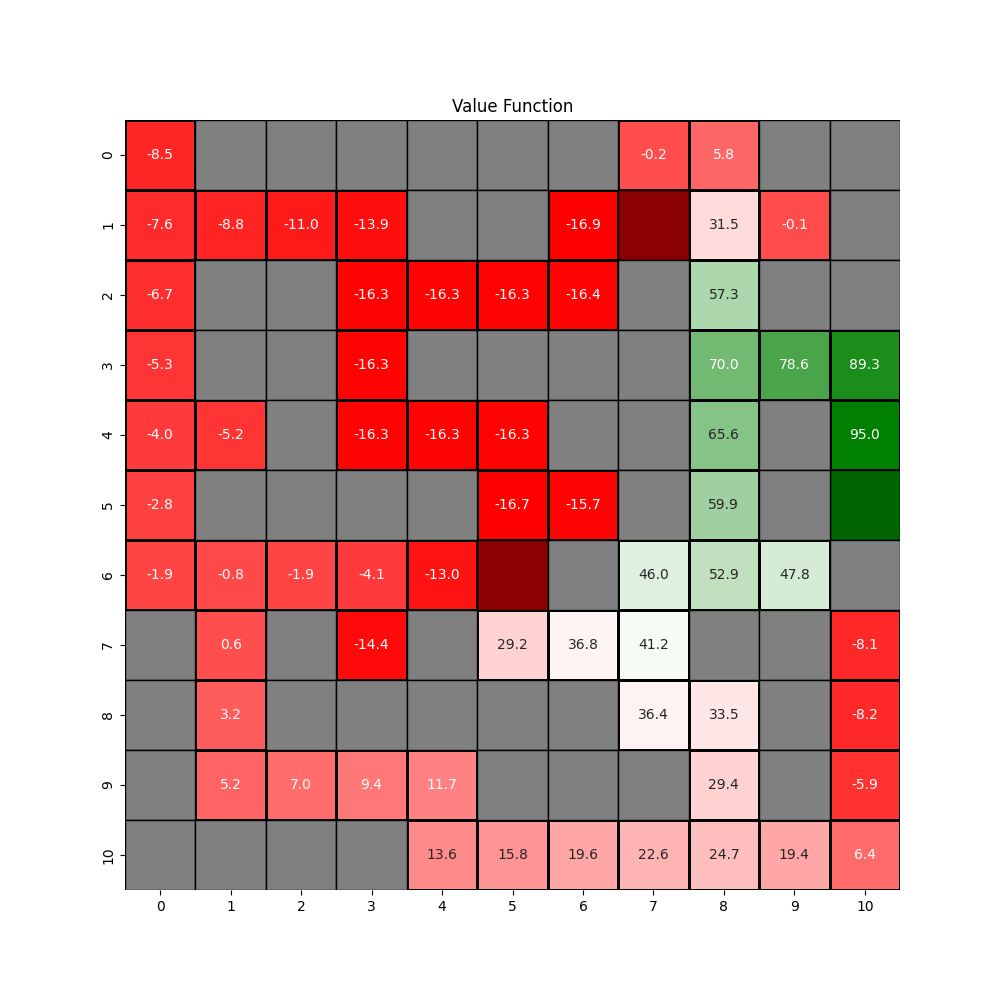
\includegraphics[width=\textwidth]{figures/value_q/default/value_function_alpha_0.1_gamma_0.95_epsilon_0.2_iteration_1000.png}
    \caption{Episode 1000.}
    \end{subfigure}\hfill
    \begin{subfigure}{0.3\textwidth}
        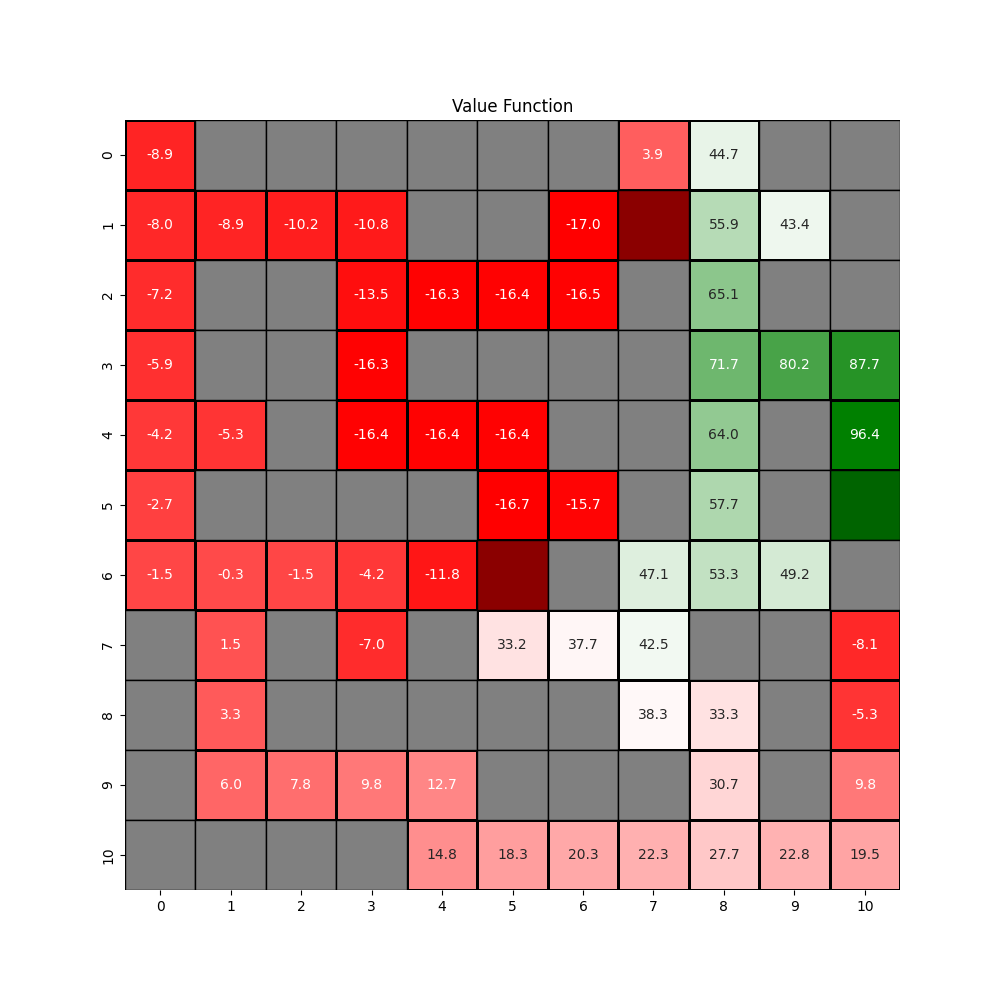
\includegraphics[width=\textwidth]{figures/value_q/default/value_function_alpha_0.1_gamma_0.95_epsilon_0.2_iteration_5000.png}
    \caption{Episode 5000}
    \end{subfigure}\hfill
    \begin{subfigure}{0.3\textwidth}
        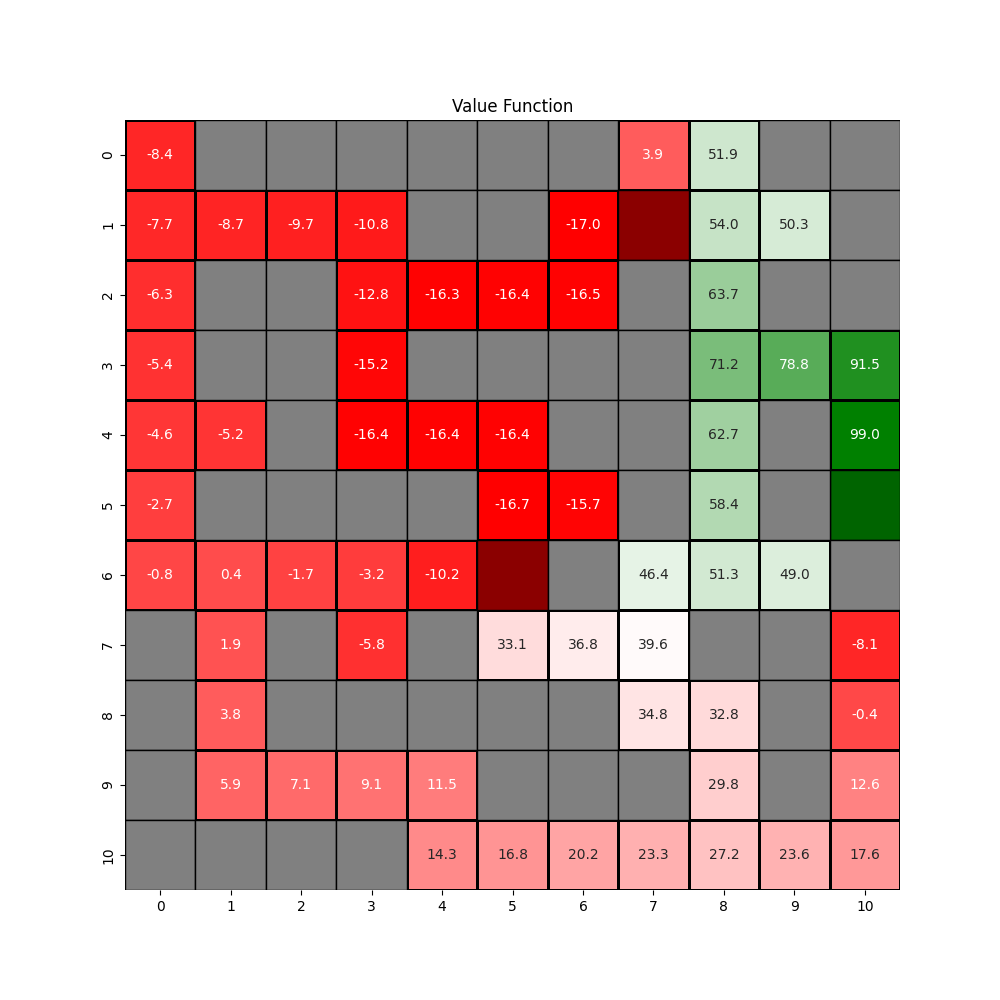
\includegraphics[width=\textwidth]{figures/value_q/default/value_function_alpha_0.1_gamma_0.95_epsilon_0.2_iteration_10000.png}
    \caption{Episode 10000}
    \end{subfigure}
    \caption{Evolution of value function throughout episodes.}
    \label{fig:default_q_learning_value}
\end{figure}







\subsection{Effect of Alpha in Temporal Difference Learning}

\subsection{Effect of Alpha in Q-Learning}

\subsection{Effect of Gamma in Temporal Difference Learning}

\subsection{Effect of Gamma in Q-Learning}

\subsection{Effect of Epsilon in Temporal Difference Learning}

\subsection{Effect of Epsilon in Q-Learning}

\section{Discussions}
\subsection{Q1}

\subsection{Q2}

\subsection{Q3}

\subsection{Q4}

\subsection{Q5}

\subsection{Q6}

\subsection{Q7}

\subsection{Q8}

\subsection{Q9}

\subsection{Q10}

\section*{Appendix}
The code set used throughout this homework is provided as follows. 

% \lstinputlisting[language=Python]{../parameter_sweep_hw2.py}



%--------------------------------------BIBLIOGRAFIA-------------------------------------------
\nocite{*} 


\end{document}

\begin{figure}[!htb]
    \centering
    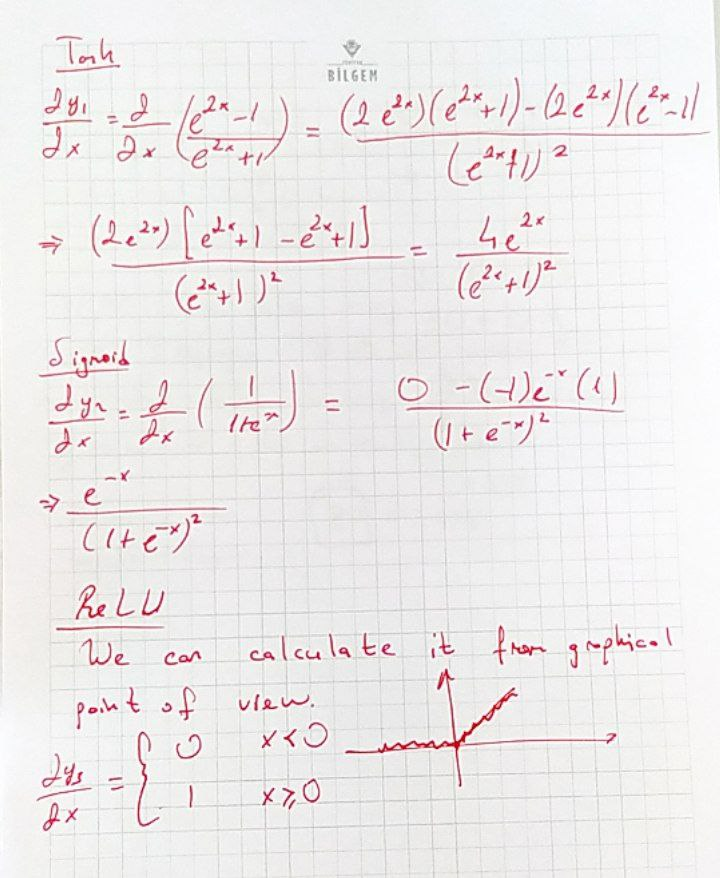
\includegraphics[width=0.6\textwidth]{figures/partial_der.jpg}
    \caption{Partial derivative calculation steps for Tanh, Sigmoid and ReLU activation functions.}
    \label{partial_der}
\end{figure}

\begin{figure}[!htb]
    \begin{subfigure}{0.5\textwidth}
        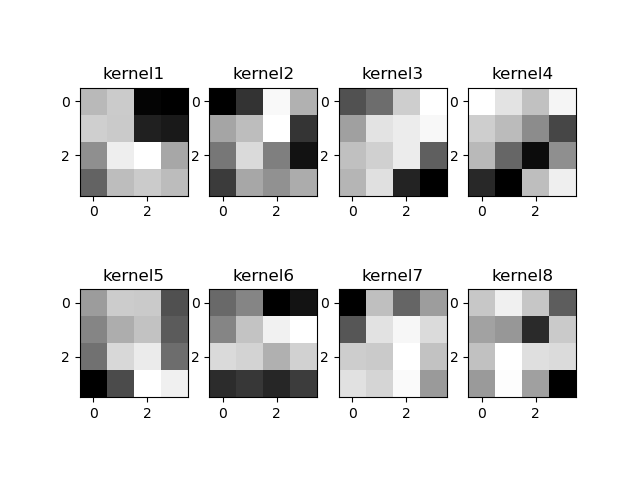
\includegraphics[width=\textwidth]{figures/q2_kernels.png}
        \caption{Kernels}
    \end{subfigure}\hfill
    \begin{subfigure}{0.5\textwidth}
        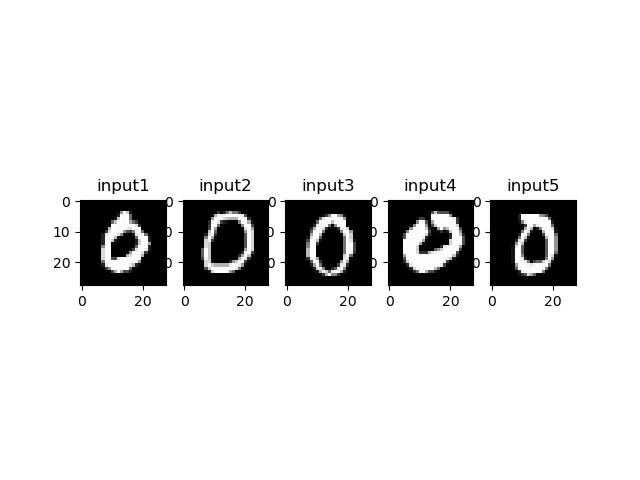
\includegraphics[width=\textwidth]{figures/q2_zero_input.png}
        \caption{Input set for number zero.}
    \end{subfigure}
    \caption{Kernel and input for number zero.}
    \label{fig:kernel_input}
\end{figure}